
We first present our motivation for using synthetic data to address data imbalance problems based on experimental findings (\Sref{sec:2.1}).
Building on these empirical insights, we propose to exploit the synthetic data (SYNAuG) as a means to uniformize the given training data distribution 
% of the given training data
(\Sref{sec:2.2}).
% Note that we do not advocate that SYNAuG is a solution for the data imbalance problem, but it provides a novel perspective from a data point of view.

\begin{figure}
    \centering
        \begin{subfigure}[b]{0.9\linewidth}
        \centering
        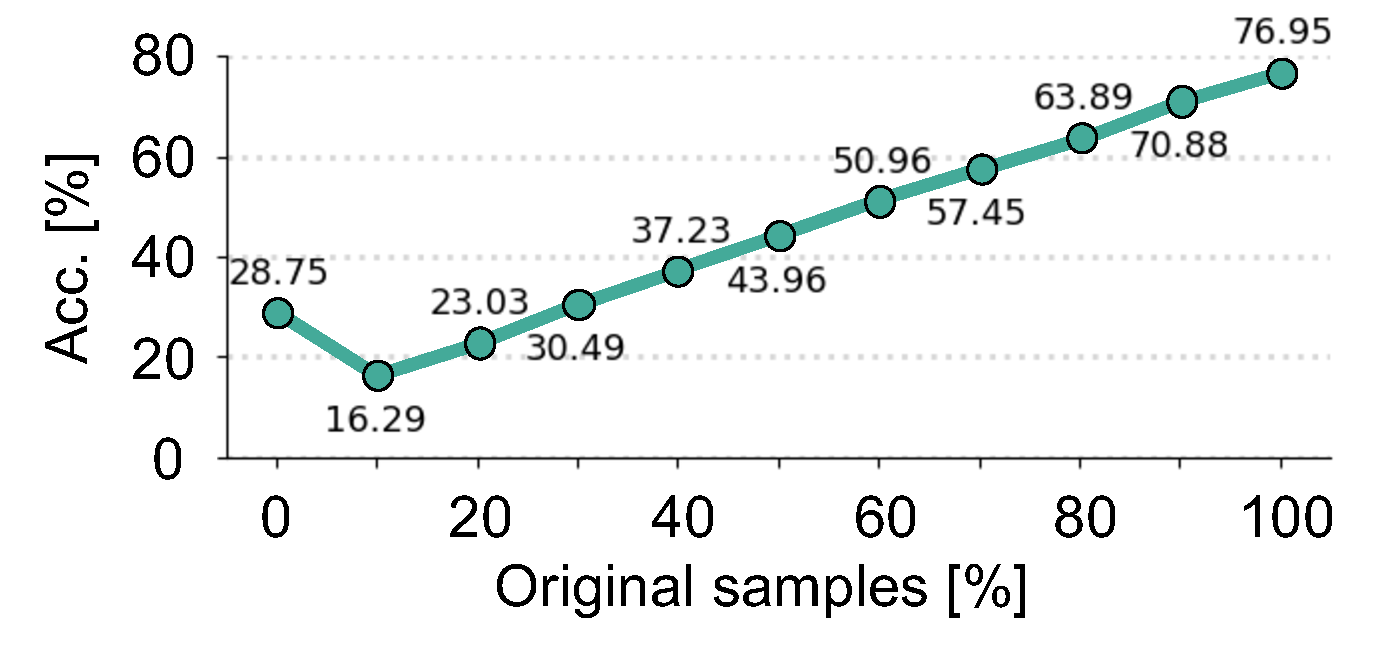
\includegraphics[width=1.0\linewidth]{figures/example1.pdf}
        \caption{Class-wise replacement}
        \label{fig:classwise}
    \end{subfigure}
    \centering
        \begin{subfigure}[b]{0.9\linewidth}
        \centering
        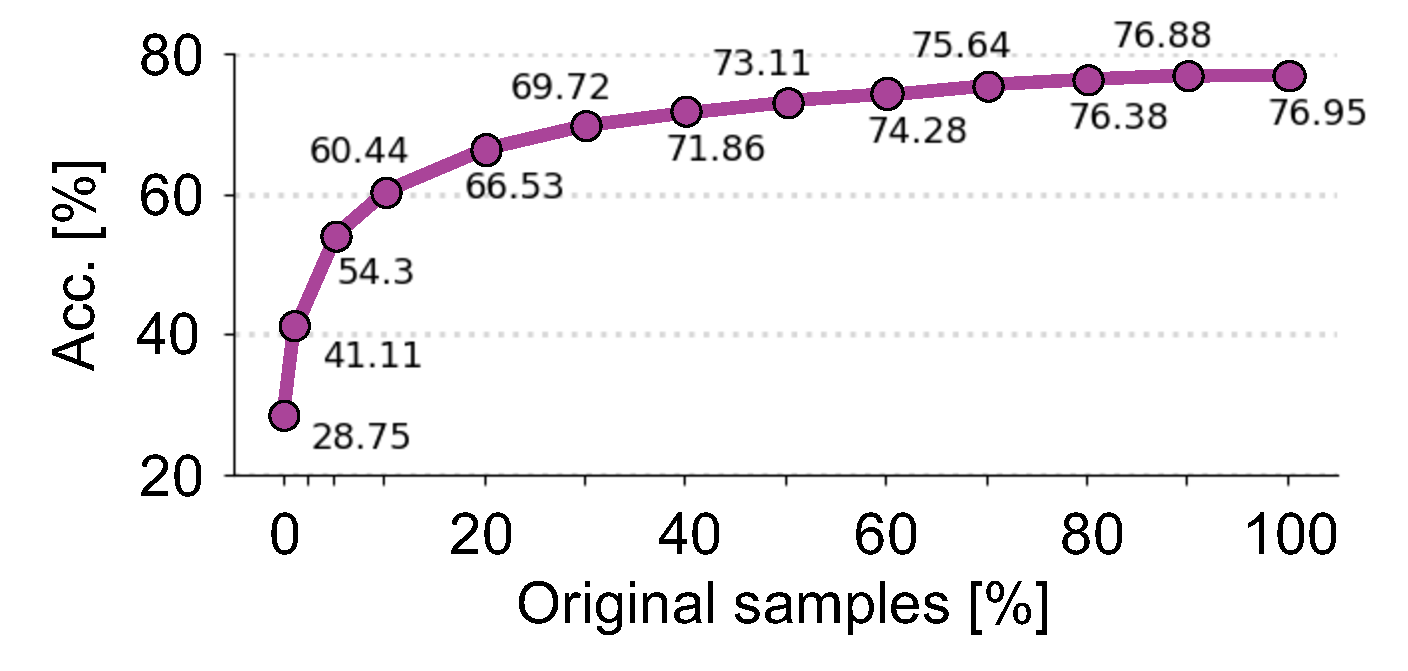
\includegraphics[width=1.0\linewidth]{figures/example2.pdf}
        \caption{Instance-wise replacement}
        \label{fig:instwise}
    \end{subfigure}    
    \caption{\textbf{Replacement test.} 
    To investigate the effect on model performance when using original and synthetic data together, we replace the original data with synthetic ones in two ways: (a) class-wise and (b) the same ratio of instances across all classes.
    We use CIFAR100, which has 500 samples per class and 100 classes.
    }
    \label{fig:abl_ratio}
\end{figure}

\subsection{Motivations}\label{sec:2.1}
During training, we consider how to curate the data, train the model, and evaluate it.
As aforementioned, prior methods addressing data imbalance problems have explored in various ways, including data re-sampling, loss function design, and model architecture.
Instead, 
% As the first step, data curation significantly affects the training and the subsequent evaluation.
we emphasize the importance of data curation and the controllability of data, as data curation significantly affects the training and the subsequent evaluation despite its position as the first step.
% In this work, we propose to utilize the power of the recent text-to-image generative model, which provides controllability in generating synthetic samples.

Before incorporating synthetic data into our proposed method, we delve into the influence of training with synthetic and original data together.
We establish two settings by controlling the ratio of original and synthetic data.
We use the generated images from the Stable Diffusion~\cite{rombach2022high} for synthetic data.
In the \textbf{first setting}, we take an extreme approach by replacing whole original data belonging to specific classes with synthetic data.
It means that certain classes have no real samples but only synthetic samples.
% , and this setting is an extreme case of data imbalance.
In the \textbf{second setting}, we uniformly replace the original data with synthetic data, which means all classes have the same ratio of original and synthetic data.
This approach ensures that every class at least has a few original data.
The significance of original samples becomes apparent through observing the performance change.

% Figure~\ref{fig:abl_ratio} shows t
The results of the two settings are in \Fref{fig:abl_ratio}.
The first setting shows the linear performance degradation as the number of classes with no original data increases (See \Fref{fig:classwise}).
However, the second setting shows the log-like performance degradation as more original data are replaced with synthetic data uniformly (See \Fref{fig:instwise}).
We achieve 41.11\% when using 1\% of real data in the second setting, which is similar to the result of 43.96\% when using 50\% of real data in the first setting.
% The performance of 1\% of real data in the second setting is 41.11\%, which is similar to the performance of 50\% of real data in the first setting, 43.96\%.
%It indicates that few original samples might be needed. and the domain gap might exist despite high-quality synthetic data.
% 어감이 few original samples 이 앵커 역할을 한다는거면 조금 더 강조를 해야할수도..
The results suggest that at least a few original samples are necessary as an anchor, as
% while
the domain gap may still exist even with high-quality synthetic data.
% In addition, the performance difference between 100\% and $n$\% accuracies in \Fref{fig:instwise} would represent the existence of the domain gap between real and synthetic data.

\begin{figure}
    \centering
        \begin{subtable}[c]{0.3\linewidth}
        \centering
        \resizebox{1.0\linewidth}{!}{
            \begin{tabular}{cc}
                \toprule
                & \textbf{Accuracy} \\ 
                \midrule
                Real  & 77.76 \\
                Syn.  & 70.56 \\
                \cmidrule{1-2}
                Total & 74.16 \\
                \bottomrule 
            \end{tabular}
        }
        \caption{Binary domain classification}    
        \label{fig:domain_cls}
    \end{subtable}
    \hspace{8mm}
    \centering
        \begin{subfigure}[c]{0.5\linewidth}
        \centering
        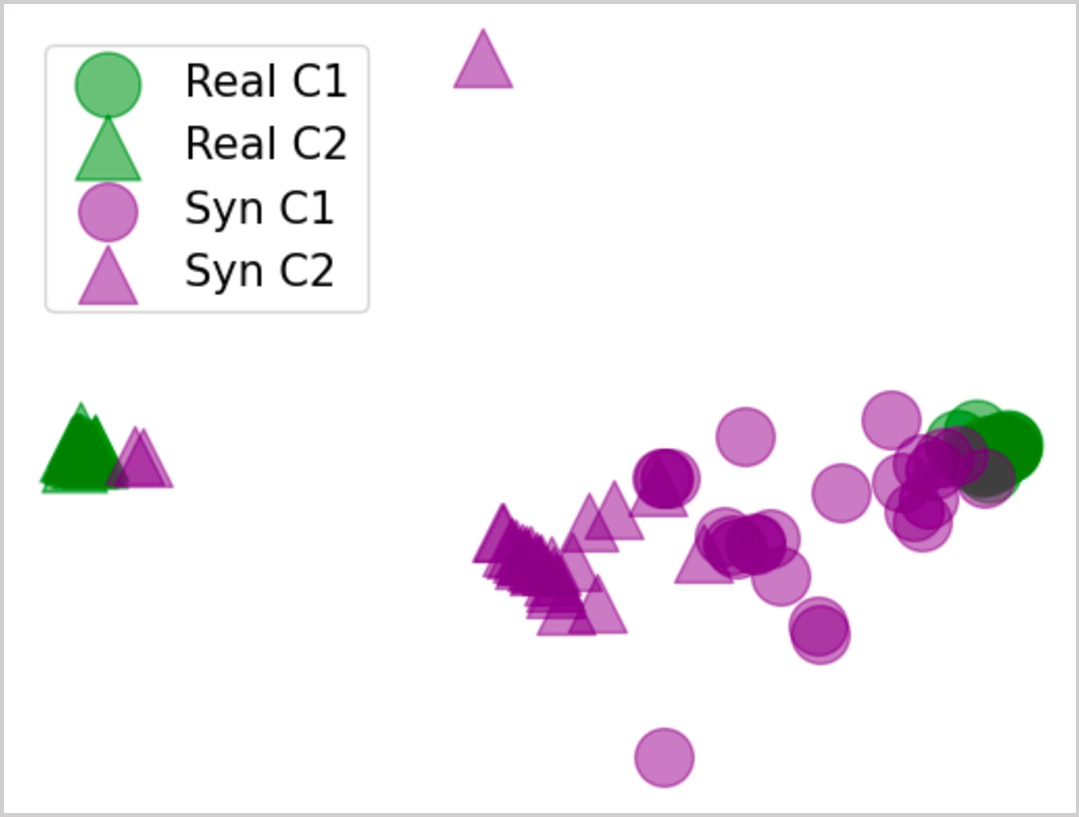
\includegraphics[width=1.0\linewidth]{figures/domain_gap.pdf}
        \caption{Feature visualization}
        \label{fig:domain_feat}
    \end{subfigure}    
    \caption{\textbf{Domain gap between real and synthetic data.} 
    We test the domain gap empirically with (a) binary domain classification and (b) feature visualization.
    For binary classification, we use 2.5k samples for each real and synthetic domain and train only one fully-connected layer with the extracted features.
    For visualization, the features are extracted from the pre-trained model on CIFAR100.
    % , a total of 5k samples.
    % We first train the model with real samples (CIFAR100) and re-train the last layer from scratch to classify the given samples as real or synthetic. 
    % For re-training, we use 2.5k samples for each real and synthetic domain, a total of 5k samples.
    % The features are extracted before the last layer.
    C1 and C2 denote different classes.
    }
    \label{fig:domain}
\end{figure}

To check the presence of a domain gap, we conduct domain classification and visualization of the features from both real and synthetic data (See \Fref{fig:domain}).
As shown in \Fref{fig:domain_cls}, the classification performance is 74.16\%.
This indicates the existence of a domain gap, considering that 50\% means no domain gap.
As shown in \Fref{fig:domain_feat}, the features of Syn C2 are more closer to Syn C1 rather than Real C2.
% the features of synthetic data in class 1 (Syn C1) are closer than features of real data. 
% \wonseok{As shown in \Fref{fig:domain_feat}, the features of synthetic data are more tightly clustered than the features of real data. }
This observation provides empirical evidence of a domain gap existing between real and synthetic data.

% If there is no domain gap between real and synthetic data, the domain classifier would be incapable of distinguishing between samples, yielding an accuracy of 50\%.
% However, as depicted in Figure \ref{fig:domain_cls}, the obtained accuracy of 74.16\% indicates a discernible domain gap.
% Visualization result depicted in \Fref{fig:domain_feat} reveals that some of the synthetic samples are distant from their corresponding real samples within the same class.
% This observation also provides empirical evidence of a domain gap existing between real and synthetic data.

In summary, (1) at least, a few real samples are important when we supplement the real samples with the synthetic samples,
(2) synthetic samples are still insufficient to fully replace the original samples, although the deep generative models show impressive performance,
thus, (3) there might be additional room for improvement due to the domain gap between the original and the synthetic data.
It is desirable that the remaining original samples serve as an anchor role, and synthetic data support and populate the insufficient samples.

% While the first case shows the linear performance degradation as shown in \Fref{fig:classwise}, the second case shows the performance degradation alleviate rather than the first case as shown in \Fref{fig:instwise}.
% Interestingly, the performance of 1\% of original data in the second case is similar to the performance of 50\% of original data in the first case.
% In addition, the performance difference between 100\% and $n$\% accuracies in \Fref{fig:instwise} would represent the existence of the domain gap between original and synthetic data in a same class.
% These results imply that (1) synthetic data is still insufficient to replace original data fully, (2) we need a few original samples when supplementing the original data with the synthetic data, and (3) there might be additional room for improvement due to the domain gap between the original and the synthetic data.
% It is desirable that the remaining original samples serve as an anchor role, and synthetic data support and populate the insufficient samples.





\subsection{SYNAuG}\label{sec:2.2}
Given the preliminary experiments, we propose SYNAuG, which leverages synthetic data to mitigate the imbalance and domain gap from the data perspective.
Our approach is applied to 
% across
three distinct tasks: long-tailed recognition, model fairness, and robustness to spurious correlation.
While these tasks differ in their ultimate objectives and evaluation metrics, the common underlying factor is the presence of data imbalance.
SYNAuG is an integrated approach designed to mitigate data imbalance across diverse tasks.

As illustrated in \Fref{fig:overview}, we first uniformize the imbalance data by generating synthetic data, train the model on the uniformized data, and finally fine-tune the last layer with a few original data uniformly subsampled from each class.
% original data.
We exploit recent powerful generative models, \eg, Stable Diffusion~\cite{rombach2022high}, to generate the synthetic data of corresponding classes or attributes with the controllable prompt.
Since they are trained on a large number of web data, it would be considered to cover and model the wide distribution of the real world.
Exploiting these favorable properties, we generate supporting data to alleviate the imbalance of the data distribution.
We generate the samples with diverse prompts like ``a photo of \{\texttt{modifier}\} \{\texttt{class}\}''.
% 개인적으로 이게 조금 더 깔끔한 느낌
%We can find the modifier by humans but use ChatGPT~\cite{ouyang2022training} to make our pipeline automatic.
We find list of proper modifiers by ChatGPT~\cite{ouyang2022training} to make our pipeline automatic.
% With the data uniformized according to the target imbalance axis, w
We train the model on uniformized data with Cross Entropy (CE) loss.

While SYNAuG is simple and effective, there is still room to improve its performance because of the domain gap identified 
% , as mentioned
in \Sref{sec:2.1}.
% because the domain gap exists between original and synthetic data, as we mentioned in \Sref{sec:2.1}.
To bring further improvement by mitigating the gap, we propose to utilize two simple methods.
% , as shown in \Fref{fig:overview}.
First, we propose to leverage
% use
Mixup~\cite{zhang2017mixup} during training to augment the samples to be interpolated samples between real and synthetic samples, \ie, domain Mixup.
Second, we propose to fine-tune the classifier on the subsampled uniform original data from the original training data after the first training stage.
% Our experiment show that t
The fine-tuned classifier would lead to more accurate recognition of the target data by alleviating the domain gap.

% 361-364에 거의 똑같은 내용이 있어서, 한번 더 써서 강조하는 느낌을 준다면 조금 더 요약하는 느낌을 주는건? To summarize, our proposed method ~
% Note that our method exploits synthetic data to address the imbalance problem from the data perspective, leveraging the data controllability of synthetic data. 
In summary, the process of SYNAuG is as follows:
%Note that based on data controllability, our method exploits the synthetic data to tackle the imbalance problem from the data point of view. The process of SYNAuG is as follows: 
(1) uniformize the original data distribution with synthetic data from the generative model, (2) train the model with uniformized data using Mixup, and (3) fine-tune the last layer with the uniformly subsampled real data.


